\scanpage{13}
\margin{$\bar{\uparrow}\ \Bigg\{\quad ?\,\begin{smallmatrix}\downarrow\\[-.5ex]\uparrow\end{smallmatrix}$}
\diagram{\begingroup\scriptsize\setlength{\arraycolsep}{1.5pt}
\setlength{\arrayrulewidth}{.22pt}
\resizebox{\linewidth}{!}{\(\begin{array}{@{}c|c|c|c|c|c@{\quad}l@{}}
\text{Notes}&\text{Notes}&\text{Notes}&\text{Notes}&\text{Notes}&\text{Notes}&\text{\begin{tikzpicture}[x=1ex,y=1ex,line width=.28pt,line cap=round]\draw (0,0)--(.75,.12)--(.07,.12);\end{tikzpicture}}\\ \cline{1-6}
1&5&7&15&20&23&\text{\begin{tikzpicture}[x=1ex,y=1ex,line width=.28pt,line cap=round]\draw (.12,0)--(.72,.10)--(.10,.10);\end{tikzpicture}}\\ \cline{1-6}
\text{\deleted{A (1976/77)}}&&&&&&\\[1.6ex]
&&&&&&\text{\begin{tikzpicture}[x=1ex,y=1ex,line width=.28pt,line cap=round]\draw (0,0)--(.82,.15)--(.08,.15);\end{tikzpicture}}\\
&&&&&&\text{\begin{tikzpicture}[x=1ex,y=1ex,line width=.28pt,line cap=round]\draw (0,0)--(.82,.10)--(.06,.08);\end{tikzpicture}}\\
\deleted{\mathrm A}\mathrm A&\mathrm B&\mathrm C&\mathrm D&\mathrm E&\mathrm E&\text{\begin{tikzpicture}[x=1ex,y=1ex,line width=.28pt,line cap=round]\draw (.15,0)--(.75,.12)--(0,.12);\end{tikzpicture}}\\ \cline{1-6}
(1976/77)&(1978/79)&(1979/80)&(1980)&(1981)&(1981)&\text{\begin{tikzpicture}[x=1ex,y=1ex,line width=.28pt,line cap=round]\draw (.15,0)--(.72,.14)--(.14,.10);\end{tikzpicture}}\\
\text{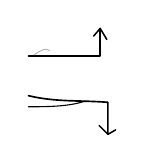
\begin{tikzpicture}[x=.014cm,y=-.014cm,line cap=round,line join=round]
\draw[line width=.55pt] (20,37)--(85,37)--(85,12);
\draw[line width=.55pt] (79,19)--(85,12)--(91,22);
\draw[gray!65,line width=.3pt] (25,36)..controls(31,32)and(36,29)..(39,32);
\draw[line width=.6pt] (20,73)..controls(45,79)and(68,77)..(92,79)--(92,108);
\draw[line width=.55pt] (84,100)--(92,108)--(99,104);
\draw[line width=.4pt] (20,83)..controls(36,83)and(56,83)..(71,78);
\end{tikzpicture}}&&&&&&\\[-.5ex]
\text{Découverte}&\text{Réveil}&\text{Die Eltern}&\text{Das Kind}&\text{Der Baumeister}&\text{Le Bâtisseur}&\\
\text{de la}&\text{en}&&&&&\\
\text{Méditation}&\text{\deleted{\unsure{C|Ca}}Cascades}&\text{(Les parents)}&\text{(L'enfant)}&\text{(Le Bâtisseur)}&&\\ \cline{1-6}
\deleted{(\unsure{\mathrm i})}&\deleted{(\unsure{\mathrm{ii}|\mathrm i})}&\deleted{(\unsure{\mathrm i|\mathrm{ii}})}&\deleted{(\unsure{\mathrm i|\mathrm{ii}})}&\deleted{(\unsure{\mathrm i|\mathrm{ii}})}&\deleted{(\unsure{\mathrm{ii}|\mathrm{iv}|\mathrm{iii}})}&\\
?\ \downarrow&\searrow&&&&&\text{\begin{tikzpicture}[x=1ex,y=1ex,line width=.28pt,line cap=round]\draw (.18,0)--(.68,.14)--(.07,.14);\end{tikzpicture}}\\
\deleted{\unsure{(\mathrm i)}}(\mathrm i)&(\mathrm{ii})&\deleted{\unsure{(}}(\mathrm i)&\deleted{(\mathrm i)}(\mathrm i)&(\mathrm i)&(\mathrm{iv})&\text{\begin{tikzpicture}[x=1ex,y=1ex,line width=.28pt,line cap=round]\draw (.10,0)--(.68,.14);\end{tikzpicture}}\\ \cline{1-6}
\text{Envol}&\text{Vers un plus long Voyage}&\text{Bild und Wahrheit}&\text{Der Wolf}&\text{Spiel- und Sucht}&\text{Le ``Maître''}&\text{\begin{tikzpicture}[x=1ex,y=1ex,line width=.28pt,line cap=round]\draw (.20,0)--(.60,.12);\end{tikzpicture}}\\
&&\text{(Image et Réalité)}&\text{(Le Loup)}&\text{(Jeu - et Fringale)}&&\\ \cline{1-6}
\text{M }1976\mathord{*}&\text{M }1979&\text{HS }\mathrm I&\text{Sch }\mathrm I&\text{Sch }\overline{\underline{\mathrm{VI}}}&\text{Sch }\overline{\underline{\mathrm{IX}}}&\text{\begin{tikzpicture}[x=1ex,y=1ex,line width=.28pt,line cap=round]\draw (.10,0)--(.50,.12);\end{tikzpicture}}
\end{array}\)}\endgroup}
% archive sheet number: 12
